\documentclass[a4paper]{article}

\usepackage[english]{babel}
\usepackage[utf8]{inputenc}
\usepackage{amsmath}
\usepackage{graphicx}
\usepackage{color}
\usepackage{float}
\usepackage{listings}
\definecolor{keywords}{RGB}{255,0,90}
\definecolor{comments}{RGB}{0,0,113}
\definecolor{red}{RGB}{160,0,0}
\definecolor{green}{RGB}{0,150,0}
\definecolor{codegreen}{rgb}{0,0.6,0}
\definecolor{codegray}{rgb}{0.5,0.5,0.5}
\definecolor{codepurple}{rgb}{0.58,0,0.82}
\definecolor{backcolour}{rgb}{0.95,0.95,0.92}
\definecolor{brown}{rgb}{0.59, 0.29, 0.0}
\definecolor{beaublue}{rgb}{0.74, 0.83, 0.9}
\definecolor{orange}{rgb}{1.0, 0.5, 0.0}
\definecolor{darkslategray}{rgb}{0.18, 0.31, 0.31}
\definecolor{deepblue}{rgb}{0,0,0.5}
\definecolor{deepred}{rgb}{0.6,0,0}
\definecolor{deepgreen}{rgb}{0,0.5,0}
\definecolor{auburn}{rgb}{0.43, 0.21, 0.1}
\definecolor{bistre}{rgb}{0.24, 0.17, 0.12}
\definecolor{babyblue}{rgb}{0.54, 0.81, 0.94}
\definecolor{ballblue}{rgb}{0.13, 0.67, 0.8}
\lstdefinestyle{myMatlabstyle}{
	language=Matlab,
	backgroundcolor=\color{white},   
	commentstyle=\color{red},
	keywordstyle=\color{black},
	identifierstyle=\color{ballblue},
	numberstyle=\tiny\color{codegray},
	stringstyle=\color{deepgreen},
	basicstyle=\footnotesize,
	breakatwhitespace=false,         
	breaklines=true,                 
	captionpos=b,                    
	keepspaces=true,                 
	numbers=left,                    
	numbersep=5pt,                  
	showspaces=false,                
	showstringspaces=false,
	showtabs=false,                  
	tabsize=2
}
\lstdefinestyle{myPythonstyle}{
	language=Python, 
	basicstyle=\ttfamily\small, 
	keywordstyle=\color{blue},
	commentstyle=\color{green},
	stringstyle=\color{red},
	showstringspaces=false,
	identifierstyle=\color{black},
}
\lstset{language=Matlab,frame=single}
\lstset{language=Python,frame=single}
\usepackage[colorinlistoftodos]{todonotes}
\usepackage[scale=0.75]{geometry}
	\title{AMATH 582 Problem Set 1: Eigenfaces}

\author{Jithin D. George}

\date{\today}

\begin{document}
\maketitle

\begin{abstract}
This homework explores the implementation of the singular value decomposition on a dataset of image files. An exploration of the application of the SVD to various kinds of images like cropped images, uncropped images and those of multiple people, yields new perspectives on the underlying features across different people.
\end{abstract}

\section{Introduction and Overview}
\label{sec:introduction}

The Singular Value Decomposition is a result from linear algebra with powerful applications. The SVD enables the decomposition of many things in a matrix format into orthogonal basis elements. Just like it is often possible to decompose a complex function into underlying eigenfunctions, we explore in a similar way, the inherent features in facial images, the eigenfaces.
 
\section{Theoretical Background}
\label{sec:theory}


The SVD of a matrix decomposes it into three matrices.
\[A=USV^{*} \]
Here, U and V represent matrices of basis elements. S is the matrix of singular values. V could be considered as the original basis matrix. U would then be the principal component basis. Since the basis elements are orthogonal and the singular value decomposition can be applied to complex matrices, both U and V are unitary matrices. With that in mind, from basic matrix arithmetic, we can get that U is an eigenvector of A*A and V is an eigenvector of AA*. Thus, the SVD is similar to the eigenvalue decomposition. However, since it is between two basis, it is not unique and exists for any matrix A.

The SVD gives a geometric interpretation of a matrix A acting on a vector V stretching it by the singular values in S along the directions of U. Finding the largest singular values with the right U and V thus essentially gives us the most important "modes" of the matrix A. Information about the weights of the modes resides in the S matrix.


\section{Implementation and Development}
The resource available to us was a vast amount of image files from UCSD's computer vision group containing both original and cropped images. The cropped images were smaller and easier to work with.

Most of the code was on extracting the information from the image files into a matrix. Each image was reshaped into a column of the matrix. Three scenarios were implemented.
\begin{itemize}
	\item Cropped images of a single person
	\item All the cropped images 
	\item Uncropped images of a single person. 
\end{itemize}

After the matrix was obtained, it was subjected to the singular value decomposition. 

Then, the three most prominent modes were looked at. After gaining information from the statistics of the singular matrix, a low rank reconstruction is attempted.





\section{Computational Results}

\subsection{Cropped images of a single person}
The singular value decomposition of a matrix containing cropped images of a single person yields the following results.

\subsubsection{The singular value matrix}
\begin{figure}[h!] 
	
	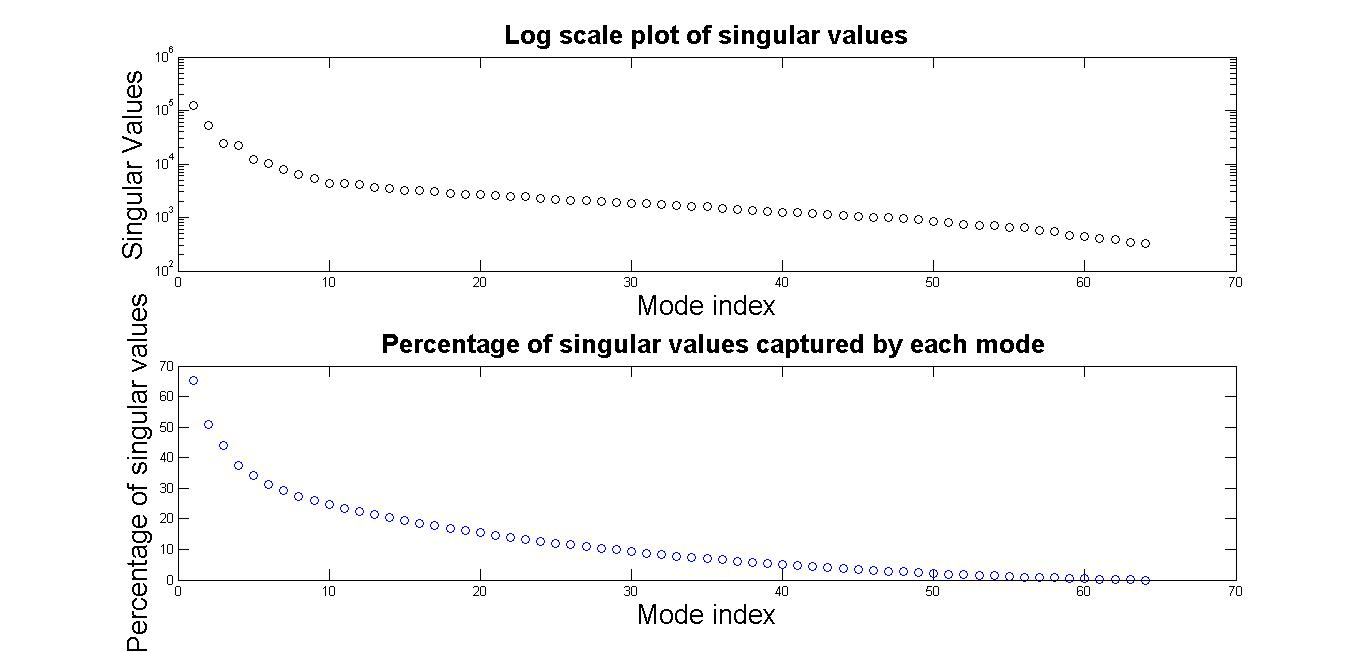
\includegraphics[width=1.\textwidth]{Crop1log.jpg}
	
	\caption{Statistics of the Singular Value Matrix}	
\end{figure}

Since the singular values don't trail to the order of $10^{-15}$, we can't ignore those values. Furthermore, to capture 90 percent of the variation, we would need around 30 modes.

\subsubsection{The first three modes}
\begin{figure}[h!] 
	
	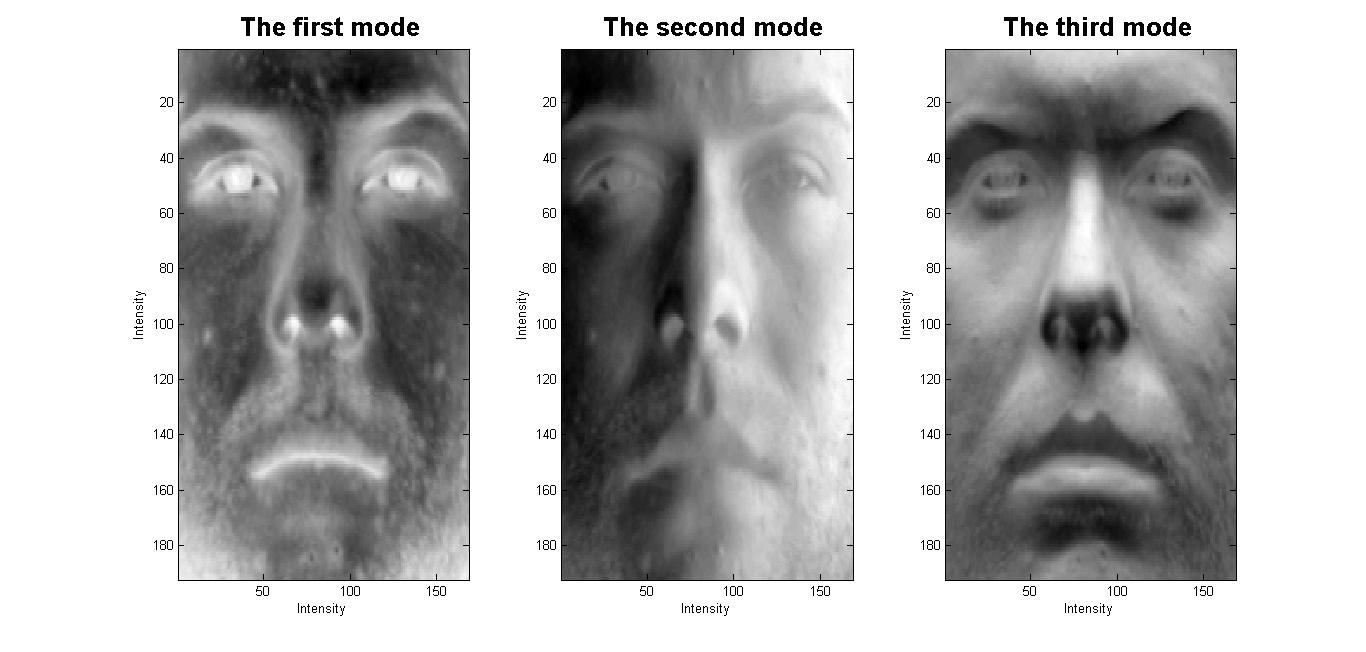
\includegraphics[width=0.91\textwidth]{modescrop1.jpg}
	
	\caption{The first 3 modes}	
\end{figure}
The first mode seems to focus on the eyes and the nostrils. The second focuses on the cheeks and the shading and in the third mode, the nose seems to be highlighted. These features contribute the most to the images of the same person under different poses and lighting.

\subsubsection{Low rank reconstruction}
\begin{figure}[H] 
	
	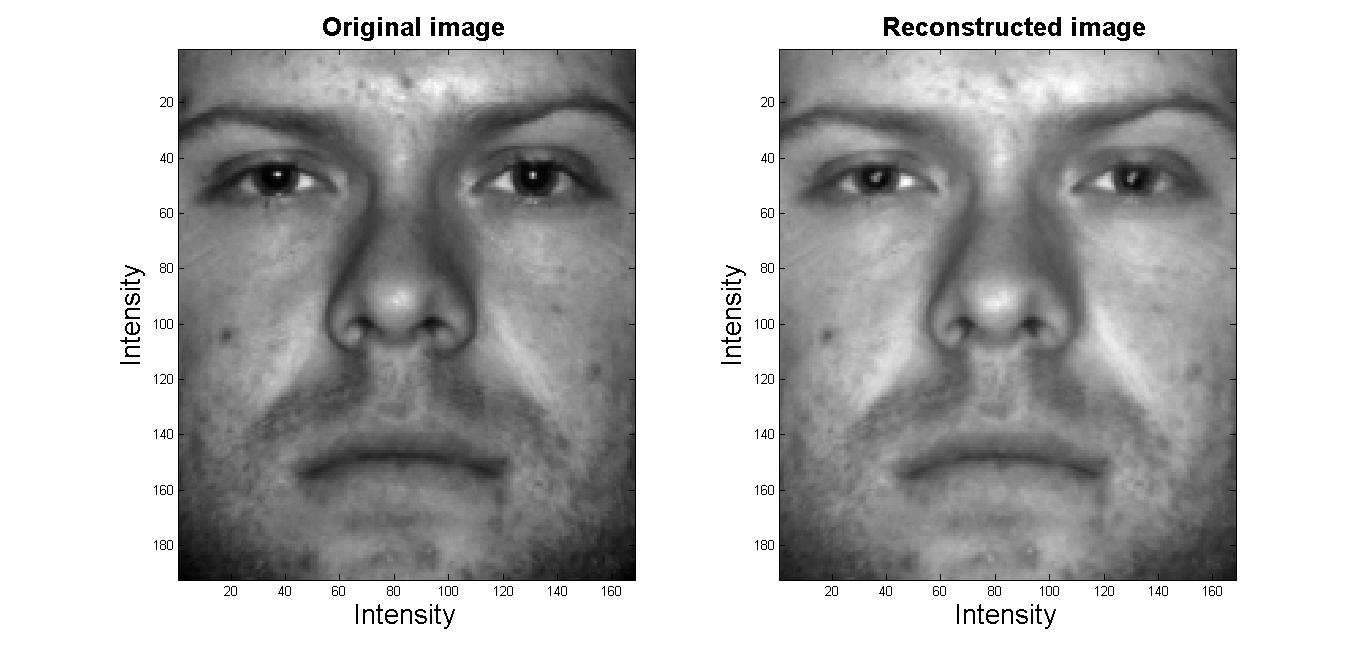
\includegraphics[width=1.\textwidth]{reconcrop130.jpg}
	
	\caption{Reconstruction of the first image with 30 modes}	
\end{figure}
The first image can be reconstructed to a good level using only 30 modes.

\subsection{All cropped images}
The singular value decomposition of a matrix containing cropped images of multiple people yields the following results.


\subsubsection{The first three modes}
\begin{figure}[h!] 
	
	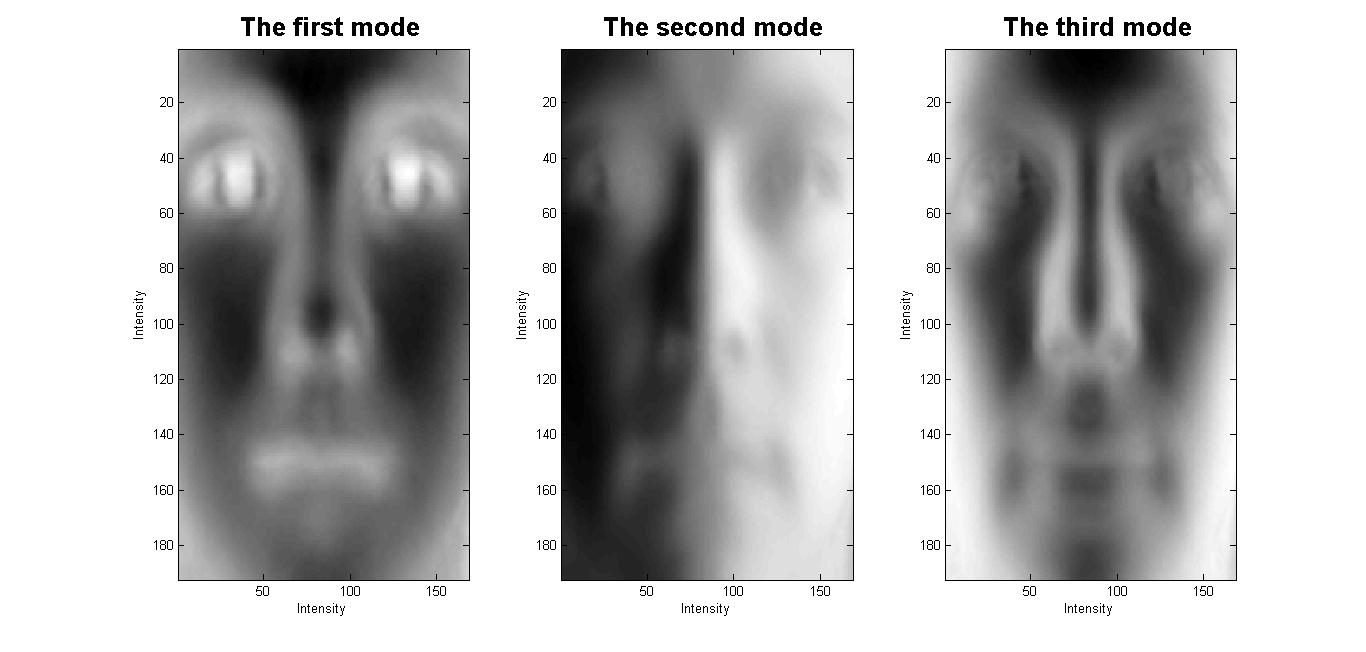
\includegraphics[width=1.\textwidth]{modesall.jpg}
	
	\caption{The first 3 modes}	
\end{figure}

Unlike the previous case, these modes look less human because they are for multiple people. Still, the eyes and the cheeks remain important features in the first two modes.

\subsubsection{Low rank reconstruction}
\begin{figure}[h!] 
	
	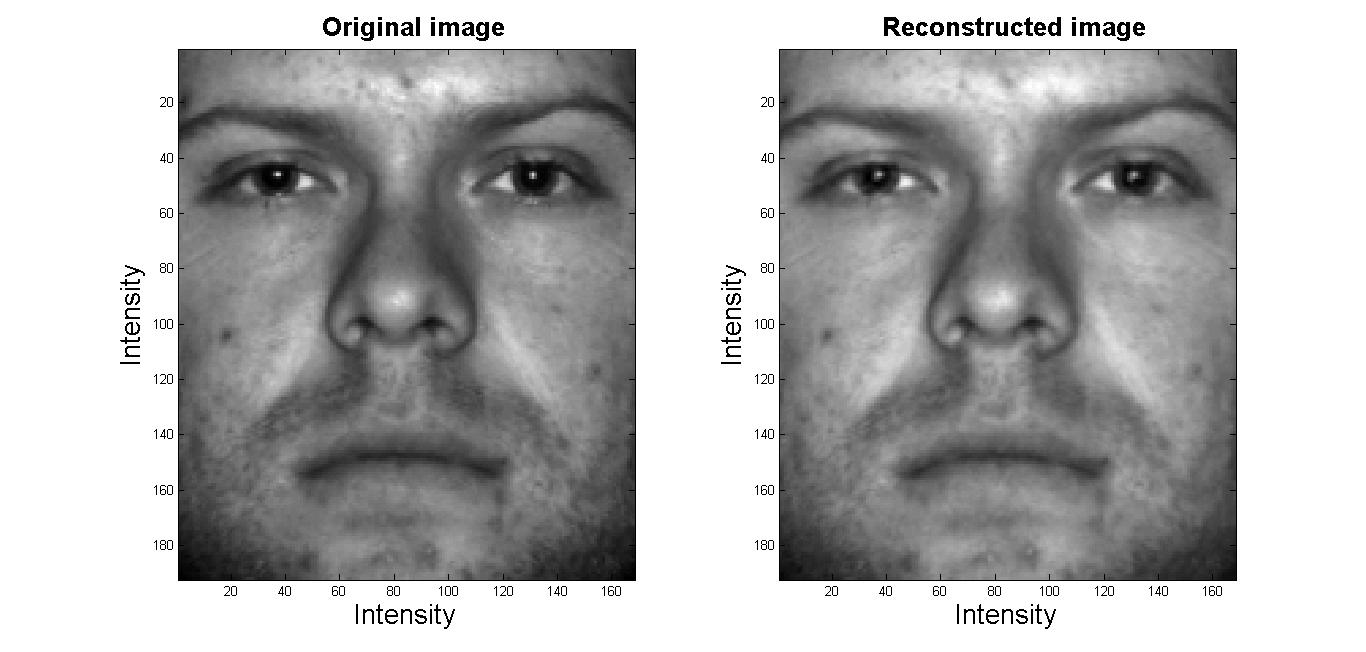
\includegraphics[width=1.\textwidth]{reconall1.jpg}
	
	\caption{Reconstruction of the first image with 800 modes}
	\end{figure}
It takes 800 modes to reconstruct the same image which only needed 30 last time. That is because these modes cater to multiple people. As a result, the following reconstruction of another image is possible with the same basis.

\begin{figure}[h!] 
	
	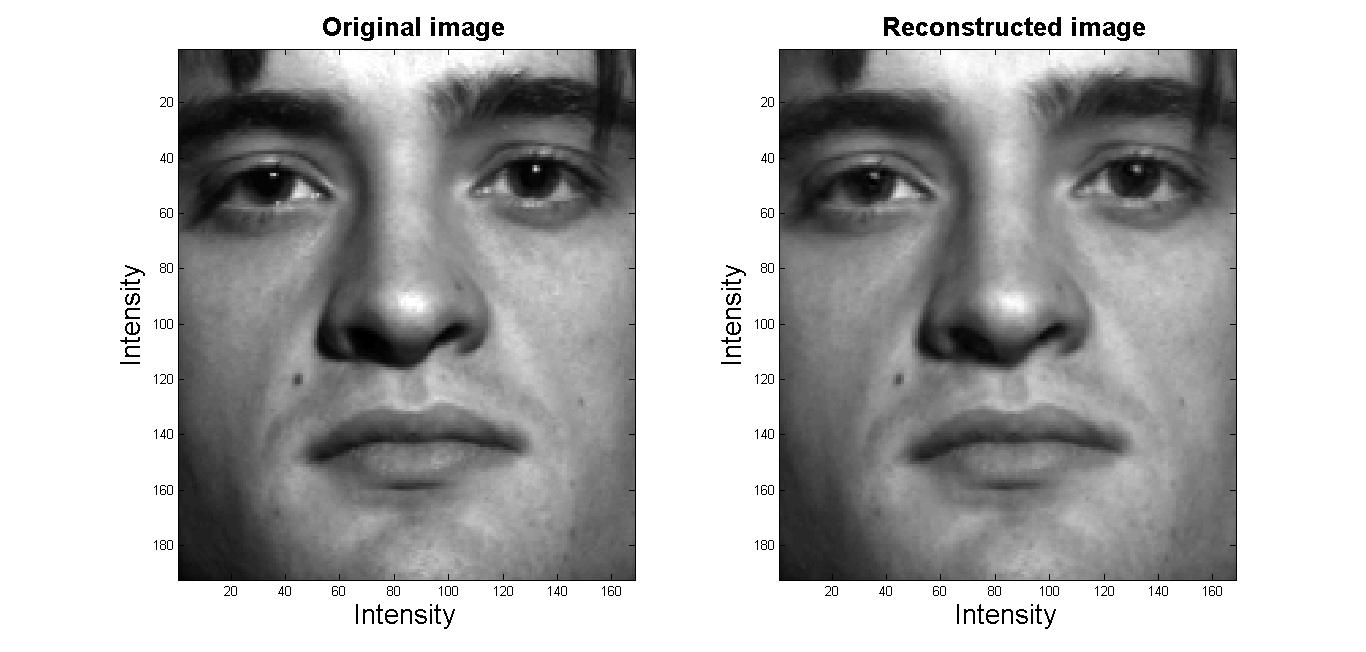
\includegraphics[width=1.\textwidth]{reconall2.jpg}
	
	\caption{Reconstruction of the 1000th image with 800 modes}
\end{figure}
\subsection{Uncropped images of a single person}
The singular value decomposition of the uncropped images of a single person yields the following results.



\subsubsection{The first three modes}
\begin{figure}[h!] 
	
	\includegraphics[width=1.\textwidth]{Uncroppmode.jpg}
	
	\caption{The first three modes}	
\end{figure}
 The biggest difference from the case of the cropped images is that the objects in the background come in the very first mode. The person and the lady in the background come in the third mode.
\subsubsection{Low rank reconstruction}
A nearly perfect reconstruction is possible with 250 modes.	
\begin{figure}[h!] 
	
	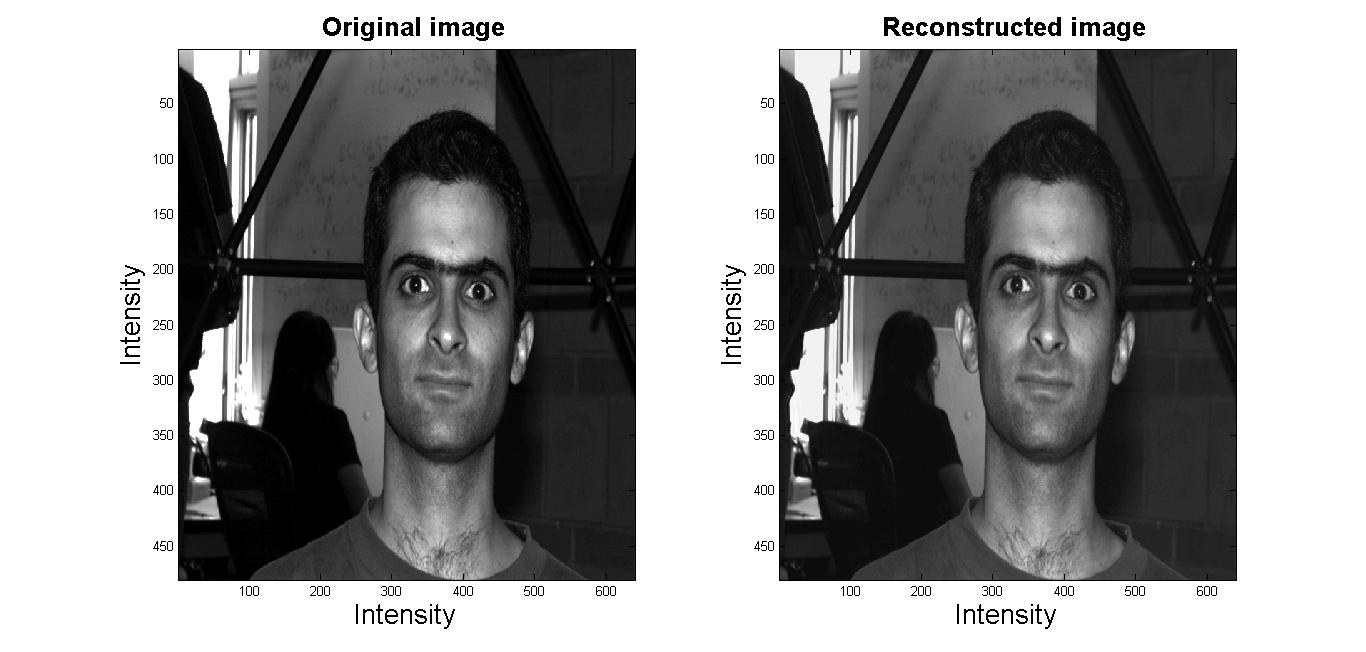
\includegraphics[width=1.\textwidth]{reconun.jpg}
	
	\caption{Reconstruction with 250 modes}	
	

\end{figure}

\section{Summary and Conclusions}
The Singular Value Decomposition is capable of accurate low-rank approximations. It does so by obtaining the basis elements with the highest singular values. The basis differs from case to case. In the case of cropped images of multiple people, the SVD created a basis which was ideal for many faces rather than one particular face. Also, in the case of uncropped images, the background found its way into the prominent modes. Finally, using modes which cover around 90 to 95 percent of the variation yields a reconstruction almost indistinguishable to the original image.

\newpage

\appendix
%dummy comment inserted by tex2lyx to ensure that this paragraph is not empty


\section{MATLAB Functions used}
\begin{itemize}
\item \textbf{[U,S,V]=svd(A): } \\ This function performs the singular value decomposition of A and returns U,S and V.
\item \textbf{imread: } \\ This function reads an image file into a matrix.
\item \textbf{reshape: } \\ This function reshapes an mxn matrix into an ixj matrix such that m*n=i*j.
\item \textbf{imagesc: } \\ This function plots a matrix as a scaled image.
\item \textbf{cumsum(p): } \\ This function finds the cumulative sum of a vector p.
\item \textbf{dir: } \\ This function list the items in a folder.
\end{itemize}

\section{MATLAB Code}
\subsection{imgextract.m}
 	\begin{lstlisting}[style=myMatlabstyle]
close all; clear all; clc;
wi=1;
for l = 1:9
	l=num2str(l);
	t=strcat('yaleB0',l);
	cd(t);
	for i=5:68
		t=dir;
		y=t(i);
		x=y.name;
		A = imread(x);
		Z(:,wi)= reshape(A,[],1);
		wi=wi+1;
	end
	cd ..
end
for l = 10:39
	if l==14
		continue
	end
	l=num2str(l);
	t=strcat('yaleB',l);
	cd(t);
	for i=5:68
		t=dir;
		y=t(i);
		x=y.name;
		A = imread(x);
		Z(:,wi)= reshape(A,[],1); 
		wi=wi+1;
	end
	cd ..
end
Z= double(Z);
[U,S,V]= svd(Z,'econ'); 
 	\end{lstlisting}
 	\subsection{imguncropped.m}
 	\begin{lstlisting}[style=myMatlabstyle]
 	close all; clear all; clc;
 	t= dir( '**.pgm');
 	wi=1;
 	for i=1:585
 	y=t(i);
 	x=y.name;
 	A = imread(x);
 	Z(:,wi)= reshape(A,[],1);
 	wi=wi+1;
 	end;
 	Z= double(Z);
 	[U,S,V]= svd(Z,'econ'); 
 	\end{lstlisting}
\subsection{plotsvd.m}
\begin{lstlisting}[style=myMatlabstyle]
%% Mode statistics
p= diag(S);
close all;
figure;
subplot(2,1,1);
semilogy(p,'ko');
f=20;
xlabel('Mode index','FontSize', f) % x-axis label
ylabel('Singular Values','FontSize', f) % y-axis label
title('\bfLog scale plot of singular values','FontSize', f)
subplot(2,1,2);
plot((1-cumsum(p)/sum(p))*100, 'bo');
xlabel('Mode index','FontSize', f) % x-axis label
ylabel('Percentage of singular values','FontSize', f) % y-axis label
title(' \bf Percentage of singular values captured by each mode','FontSize', f)

%% First three modes
figure;
m= 480;
n=640;
U1= reshape(U(:,1),m,n);
subplot(1,3,1);
colormap('gray'); imagesc(U1);
xlabel('Intensity') % x-axis label
ylabel('Intensity') % y-axis label
title(' \bf The first mode','FontSize', f)
subplot(1,3,2);
U2= reshape(U(:,2),m,n);
colormap('gray'); imagesc(U2);
xlabel('Intensity') % x-axis label
ylabel('Intensity') % y-axis label
title(' \bf The second mode','FontSize', f)
subplot(1,3,3);
U3= reshape(U(:,3),m,n);
colormap('gray'); imagesc(U3);
xlabel('Intensity') % x-axis label
ylabel('Intensity') % y-axis label
title(' \bf The third mode','FontSize', f)

%% Reconstruction
j=300;
R= U(:,1:j)*S(1:j,1:j)*V(:,1:j)';

R1= reshape(R(:,1),m,n);
figure;
subplot(1,2,2);
colormap('gray'); imagesc(R1);
xlabel('Intensity','FontSize', f) % x-axis label
ylabel('Intensity','FontSize', f) % y-axis label
title(' \bf Reconstructed image','FontSize', f)

subplot(1,2,1);
Z1= reshape(Z(:,1),m,n);
colormap('gray'); imagesc(Z1);
xlabel('Intensity','FontSize', f) % x-axis label
ylabel('Intensity','FontSize', f) % y-axis label
title(' \bf Original image','FontSize', f)
\end{lstlisting}
\end{document}